\documentclass{article}
\usepackage[utf8]{inputenc}
\usepackage[polish]{babel}
\usepackage{graphicx}
\usepackage[T1]{fontenc}
\usepackage{wrapfig}
\usepackage{fancyhdr}
\usepackage{tabularx}
\usepackage{hyperref}




%\usepackage[a4paper,top=2cm,bottom=2cm,left=3cm,right=3cm,marginparwidth=1.75cm]{geometry}
\usepackage[includeheadfoot,
            left=1in,
            right=1in,
            top=1cm,
            bottom=1cm,
            headheight=1cm]{geometry}


\pagestyle{fancy}
\fancyhf{}
\renewcommand{\headrulewidth}{0pt}
\renewcommand{\footrulewidth}{0pt}

\fancypagestyle{firstpage}
{
    \fancyhead[L]       % <-----------------LEWA STRONA-----------------
        {

            \vspace{0.25cm}
            \textbf{\textit{Miłosz Grześkowiak}} \\
            {\textit{Rok 1 Informatyka Stosowana i Systemy Pomiarowe}} \\
            {\textit{17 Marca 2025}} \\
        }


    \fancyhead[R]   % <---------------------PRAWA STRONA------------
        {

             \vspace{0.25cm}
             \textit{18 Marca 2025}  \\
             {Prowadząca: } \\
             {\textit{dr Sylwia Owczarek}} \\

        }
}
\begin{document}
\textbf{ }\\
\textbf{ }\\
\thispagestyle{firstpage}
\centering
\section*{Ćwiczenie nr. 7}
\subsection*{Temat: Badanie drgań wahadła skrętnego (torsyjnego)}
\textbf{ }\\
\textbf{ }\\
\textbf{ }\\
\textbf{ }\\
\begin{tabularx}{0.8\textwidth} {
  | >{\centering\arraybackslash}X |     % 1  }
  | >{\centering\arraybackslash}X |     % 2  }   LICZBA
  | >{\centering\arraybackslash}X |     % 3  }   KOLUMN
  | >{\centering\arraybackslash}X |}    % 4  }
 \hline


 %---------------------------OPIS-------------------------------
 \#
 & 1. Długość pręta [cm]
 & 2. Średnica pręta [mm]
 & 3. Długość 20 okresów [s]  \\
%---------------------------OPIS-------------------------------


\hline
\hline
%---------------------------DANE-------------------------------
\hline 1 & 31.0 & 3.44 & 12.91 \\
\hline 2 & 31.0 & 3.44 & 13.38 \\
\hline 3 & 31.1 & 3.42 & 13.06 \\
\hline 4 & 31.0 & 3.43 & 12.94 \\
\hline 5 & 31.1 & 3.43 & 13.00 \\
\hline Średnia & 30.84 & 3.432 & 13.058 \\
%---------------------------DANE-------------------------------
\hline
\end{tabularx}

\textbf{ }\\
\textbf{ }\\
\textbf{ }\\


\raggedright
    {
        {Dokładność wartości z pomiaru 1} \\
        {$\Delta_1$= 0.1cm}\\
        \textbf{ }\\
        {Dokładność wartości z pomiaru 2} \\
        {$\Delta_2$= 0.01mm}\\
        \textbf{ }\\
        {Dokładność wartości z pomiaru 3} \\
        {$\Delta_3$= 0.01s}\\
        \textbf{ }\\
    }

\centering

\begin{tabularx}{0.8\textwidth} {
  | >{\centering\arraybackslash}X |     % 1  }
  | >{\centering\arraybackslash}X |     % 2  }   LICZBA
  | >{\centering\arraybackslash}X |     % 3  }   KOLUMN
  | >{\centering\arraybackslash}X |
  | >{\centering\arraybackslash}X |}    % 4  }
 \hline


 %---------------------------OPIS-------------------------------
 \#
 & 1. Masa kulki 1 [g]
 & 2. Średnica kulki 1 [mm]
 & 3. Masa kulki 2 [g]
 & 4. Średnica kulki 2 [mm] \\
%---------------------------OPIS-------------------------------


\hline
\hline
%---------------------------DANE-------------------------------
\hline 1 & 31.9 & 20.32 & 63.3 & 25.05 \\
\hline 2 & 31.9 & 20.31 & 63.3 & 25.17 \\
\hline 3 & 31.9 & 20.34 & 63.3 & 25.16 \\
\hline 4 & 31.9 & 20.34 & 63.3 & 25.17 \\
\hline 5 & 31.9 & 20.34 & 63.3 & 25.16 \\
\hline Średnia & 31.90 & 20.330 & 63.30 & 25.142 \\
%---------------------------DANE-------------------------------
\hline
\end{tabularx}

\textbf{ }\\
\textbf{ }\\

\raggedright
    {
        {Dokładność wartości z pomiaru 1,3} \\
        {$\Delta_{13}$= 0.1g}\\
        \textbf{ }\\
        {Dokładność wartości z pomiaru 2,4} \\
        {$\Delta_{24}$= 0.01mm}\\
        \textbf{ }\\
    }

\centering

\begin{tabular}{|c|c|c|c|c|c|c|}
\hline
\multirow{}{}{} & \multicolumn{3}{c|}{Długość 20 okresów [s] dla r = 10.18mm} & \multicolumn{3}{c|}{Długość 20 okresów [s] dla r = 12.57mm} \\ \cline{2-7}
\# & Pom. 1 & Pom. 2 & Średnia & Pom. 1 & Pom. 2 & Średnia \\ \hline
d = r + 1cm & 14.00 & 14.09 & 14.04 & 14.93 & 14.85 & 14.89 \\ \hline
d = r + 2cm & 14.84 & 14.93 & 14.88 & 16.53 & 16.38 & 16.45 \\ \hline
d = r + 3cm & 16.07 & 15.93 & 16.00 & 18.34 & 18.50 & 18.42 \\ \hline
d = r + 4cm & 17.38 & 17.28 & 17.33 & 20.53 & 20.53 & 20.53 \\ \hline
d = r + 5cm & 18.93 & 18.75 & 18.84 & 23.25 & 22.84 & 23.05 \\ \hline
d = r + 6cm & 20.65 & 20.35 & 20.50 & 25.44 & 25.41 & 25.43 \\ \hline
d = r + 7cm & 22.38 & 22.22 & 22.30 & 28.18 & 28.22 & 28.20 \\ \hline
d = r + 8cm & 23.68 & 23.72 & 23.70 & 31.19 & 31.13 & 31.16 \\ \hline
d = r + 9cm & 25.66 & 25.50 & 25.58 & 33.69 & 33.69 & 33.69 \\ \hline
d = r + 10cm & 27.78 & 27.79 & 27.79 & 36.78 & 36.47 & 36.63 \\ \hline
\end{tabular} \\

\textbf{} \\
\textbf{} \\

\raggedright
    {
    {Dokładność wartości z pomiarów} \\
    {$\Delta = 0.01s$} \\
    \textbf{} \\
    }

\textbf{ }\\
\textbf{ }\\


\pagebreak


\centering

\section*{ZAGADNIENIA TEORETYCZNE}

{Wahadło skrętne (torsyjne) to układ fizyczny, który służy do badania drgań harmonicznych bryły sztywnej zawieszonej na elastycznym pręcie lub drucie. Głównym celem eksperymentu jest wyznaczenie okresu drgań wahadła torsyjnego oraz określenie momentu kierującego \( D \), który charakteryzuje właściwości sprężyste pręta. Aby zrozumieć zasady działania wahadła torsyjnego, należy odwołać się do kilku kluczowych zagadnień z mechaniki klasycznej.

\subsection*{1. Ruch bryły sztywnej wokół środka masy}
Bryła sztywna to ciało, którego punkty materialne pozostają w stałych odległościach względem siebie. Ruch obrotowy bryły sztywnej wokół środka masy opisuje się za pomocą równania ruchu obrotowego:

\[
\tau = I \alpha
\]

gdzie:
\begin{itemize}
    \item \(\tau\) – moment siły działający na bryłę,
    \item \(I\) – moment bezwładności bryły względem osi obrotu,
    \item \(\alpha\) – przyspieszenie kątowe.
\end{itemize}

W przypadku wahadła torsyjnego, moment siły jest proporcjonalny do kąta skręcenia pręta, co prowadzi do ruchu harmonicznego.

\subsection*{2. Moment bezwładności}
Moment bezwładności \( I \) jest miarą bezwładności bryły w ruchu obrotowym. Zależy on od rozkładu masy względem osi obrotu i jest określony wzorem:

\[
I = \int r^2 \, dm
\]

gdzie \( r \) to odległość elementu masy \( dm \) od osi obrotu. Dla prostych brył geometrycznych momenty bezwładności są znane i można je znaleźć w tablicach fizycznych.

\subsection*{3. Twierdzenie Steinera}
Twierdzenie Steinera (twierdzenie o osiach równoległych) pozwala obliczyć moment bezwładności bryły względem dowolnej osi, jeśli znany jest moment bezwładności względem osi przechodzącej przez środek masy. Twierdzenie to ma postać:

\[
I = I_{\text{cm}} + md^2
\]

gdzie:
\begin{itemize}
    \item \( I_{\text{cm}} \) – moment bezwładności względem osi przechodzącej przez środek masy,
    \item \( m \) – masa bryły,
    \item \( d \) – odległość między osiami.
\end{itemize}

\subsection*{4. Budowa i zasada działania wahadła torsyjnego}
Wahadło torsyjne składa się z bryły sztywnej (np. dysku lub pręta) zawieszonej na elastycznym pręcie lub drucie. Gdy bryła zostanie skręcona o pewien kąt \( \theta \), pręt działa na nią momentem siły sprężystej, który dąży do przywrócenia równowagi. Moment ten jest proporcjonalny do kąta skręcenia:

\[
\tau = -D \theta
\]

gdzie \( D \) to moment kierujący, który zależy od właściwości sprężystych pręta.

\subsection*{5. Okres drgań harmonicznych wahadła torsyjnego}
Ruch wahadła torsyjnego jest ruchem harmonicznym, a jego okres \( T \) zależy od momentu bezwładności \( I \) oraz momentu kierującego \( D \). Okres drgań można wyrazić wzorem:

\[
T = 2\pi \sqrt{\frac{I}{D}}
\]

gdzie:
\begin{itemize}
    \item \( T \) – okres drgań,
    \item \( I \) – moment bezwładności bryły względem osi obrotu,
    \item \( D \) – moment kierujący.
\end{itemize}

\subsection*{6. Wzór na okres drgań wahadła skrętnego i moment kierujący \( D \)}
Moment kierujący \( D \) jest związany z właściwościami sprężystymi pręta i można go wyznaczyć na podstawie okresu drgań \( T \) oraz momentu bezwładności \( I \):

\[
D = \frac{4\pi^2 I}{T^2}
\]

Wartość \( D \) zależy od materiału pręta, jego długości oraz średnicy. Dla pręta o długości \( L \) i module sztywności \( G \), moment kierujący można również wyrazić jako:

\[
D = \frac{G J}{L}
\]

gdzie \( J \) to moment bezwładności przekroju pręta względem osi skręcania.}

\section*{OPIS DOŚWIADCZENIA}

{Eksperyment polegał na sprawdzeniu jak obciążenie metalowego pręta, wpłynie na jego okres drgań. W tym celu skorzystano z metalowego pręta zawieszonego na drucie, dwóch zestawów kulek, o masie 31.9g i 63.3g, stopera oraz elektromagnesu. Następnie sprawdzano jak odległość kulek na pręcie wpłynie na jego okres wahań. Pomiary wykonano kilkukrotnie, dla kilku odległości $d$ od środka pręta, oraz dla dwóch różnych zestawów kulek.} \\

\section*{OPRACOWANIE WYNIKÓW POMIARÓW}

{Posiadając wartości długości, średnicy i długości 20 okresów pręta, masę i średnice kulek oraz długość 20 okresów dla różnych odległości kulek, możemy oszacować wartości takie jak:
\begin{itemize}
    \item Masa pręta
    \item Moment bezwładności pręta
    \item Wartość momentu kierującego
\end{itemize}

\subsection*{Masa pręta}
Masę pręta możemy obliczyć za pomocą wzoru:
\[m_p=\rho*V=\rho*\frac{\pi}{4}*l*\phi^2\]
Gdzie:
\begin{itemize}
    \item $m_p$ - Masa pręta
    \item $\rho$ - Gęstość materiału pręta (stal - $7.9\frac{g}{cm^3}$
    \item $l$ - Długość pręta
    \item $\phi$ - Średnica pręta
\end{itemize}
A więc:
\[m_p = 7.9\frac{g}{cm^3}*\frac{\pi}{4}*30.84cm*(0.343cm)^2\approx22.538g\]

\subsection*{Moment bezwładności pręta}
Moment bezwładności możemy obliczyć za pomocą wzoru:
\[I_p=\frac{1}{12}*m_p*l^2\]
Gdzie:
\begin{itemize}
    \item $I_p$ - Moment bezwładności pręta
    \item $m_p$ - Masa pręta
    \item $l$ - Długość pręta
\end{itemize}
Więc:
\[I_p = \frac{1}{12}*22.538g*(30.84cm)^2\approx1786.335g*cm^2\]

\subsection*{Wartość momentu kierującego}
Wartość momentu kierującego możemy obliczyć za pomocą wzoru:
\[D = \frac{\pi^3*l^3*\phi^2*\rho}{12*T_p^2}\]
Gdzie:
\begin{itemize}
    \item $D$ - Wartość momentu kierującego
    \item $l$ - Długość pręta
    \item $\phi$ - Średnica pręta
    \item $\rho$ - Gęstość materiału pręta
    \item $T_p$ - Okres drgań pręta bez kul
\end{itemize}
Więc:
\[D = \frac{\pi^3*(30.84cm)^3*(0.3432cm)^2*7.9\frac{g}{cm^3}}{12*(0.6539s)^2}\approx164.934*10^3N*m\]

\subsection*{Wykresy oraz regresja}
Możemy określić jak będzie wyglądał wykres długości 20 okresów w zależności od odległości środka ciężkości. Pomogą nam w tym wzory na współczynniki prostej $y = Ax + B$. Wzory na te współczynniki wyglądają następująco:
\[A = \frac{8*\pi^2*m_k}{D}\]
\[B = \frac{\pi}{3*D}*m_p*l^2+\frac{16*\pi^2}{5*D}*m_k*R_k^2\]
Gdzie:
\begin{itemize}
    \item $m_k$ - Masa kulki
    \item $D$ - Wartość momentu kierującego
    \item $m_p$ - Masa pręta
    \item $l$ - Długość pręta
    \item $R_k$ - Promień kulki
\end{itemize}
\textbf{} \\
\textbf{} \\
Podstawiając odpowiednie wartości do wzoru wychodzi nam: \\
Dla kulki 1:
\[A = \frac{8*\pi^2*31.90g}{164.934*10^3N*m} \approx 0.015\]
\[B = \frac{\pi}{3*164.934*10^3N*m}*22.538g*(30.84cm)^2+\frac{16*\pi^2}{5*164.934*10^3N*m}*31.90g*(1.018cm)^2 \approx 0.142\]
\textbf{} \\
Dla kulki 2:
\[A = \frac{8*\pi^2*63.30g}{164.934*10^3N*m} \approx 0.030\]
\[B = \frac{\pi}{3*164.934*10^3N*m}*22.538g*(30.84cm)^2+\frac{16*\pi^2}{5*164.934*10^3N*m}*63.30g*(1.257cm)^2 \approx 0.155\]

\textbf{} \\
\textbf{} \\
Z czego wynika, że końcowe wzory na funkcję wynoszą:
\[y_1=0.023x_1+0.218\]
\[y_2=0.046x_2+0.238\]

\subsection*{Regresja liniowa}
Regresję liniową możemy obliczyć za pomocą metody najmniejszych kwadratów korzystając ze wzorów:
\[a=\frac{n\sum^n_{i=1}(x_iy_i)-\sum^n_{i=1}(x_i)\sum^n_{i=1}(y_i)}{n\sum^n_{i=1}(x_i^2)-(\sum^n_{i=1}(x_i))^2}\]
\[b = \frac{\sum^n_{i=1}(y_i)-a\sum^n_{i=1}(x_i)}{n}\]
Możemy znaleźć współczynniki funkcji liniowej $y = ax+b$ \\
Obliczenia współczynników regresji liniowej zostały wykonane w autorskim skrypcie w języku $Python^{[1]}$ (patrz przypis) \\
\textbf{} \\
\textbf{} \\
Wykresy zostały zamieszczone na samym końcu sprawozdania.  \\
Pierwszy wykres zawiera regresję liniową obliczoną za pomocą wzorów podanych w opisie ćwiczenia:
\[A = \frac{8*\pi^2*m_k}{D}\]
\[B = \frac{\pi}{3*D}*m_p*l^2+\frac{16*\pi^2}{5*D}*m_k*R_k^2\]
Drugi wykres zawiera regresję liniową obliczoną za pomocą skryptu w języku $Python^{[1]}$. \\
\textbf{} \\
Zauważalnym, a jednocześnie zaskakującym zjawiskiem jest fakt, że regresja liniowa obliczona metodą najmniejszych kwadratów jest dokładniejsza niż metoda podana w opisie ćwiczenia.
}\\





\section*{WNIOSKI}

{
Wnioskując z powyższych obliczeń, oraz wykresów, można stwierdzić, że: \\
\textbf{} \\
Odległość obciążników od środka ciężkości jest wprost proporcjonalna do długości jednego okresu drgań wahadła skrętnego. \\
oraz \\
Masa obciążników jest wprost proporcjonalna do długości jednego okresu drgań wahadła skrętnego. \\
\textbf{} \\
\textbf{} \\
Ciekawym zjawiskiem jest fakt wspomniany w podrozdziale "Regresja Liniowa", gdzie regresja obliczona metodą najmniejszych kwadratów jest dokładniejsza niż metoda polegająca na wyliczeniu regresji z danych związanych z ćwiczeniem. \\
Metoda najmniejszych kwadratów jednak opiera się na samych punktach zmierzonych przez człowieka, zaś metoda polegająca na wyliczeniu regresji z danych, nie bierze pod uwagę zjawisk współistniejących. \\
Może być to związane z takimi zjawiskami jak:
\begin{itemize}
    \item \textbf{Opór powietrza} - okres drgań pręta mógł zostać spowolniony przez opór powietrza.
    \item \textbf{Błąd pomiarowy} - narzędzia pomiarowe takie jak chociażby stoper mogły być rozregulowane i podawać błędne wyniki.
    \item \textbf{Błąd ludzki} - wyniki mogły zostać błędnie zmierzone bądź odczytane przez wykonujących ćwiczenie.
\end{itemize}
\textbf{} \\
\textbf{} \\
W przyszłości wykonując ćwiczenie, można wykonać obliczenia uwzględniające opór powietrza, oraz wykonać pomiary różnymi narzędziami pomiarowymi.
}

\subsection*{Przypisy}
\begin{enumerate}
    \item {\href{https://github.com/milosz0542/I-Pracownia-Fizyczna}{https://github.com/milosz0542/I-Pracownia-Fizyczna}}
    \begin{itemize}
        \item Regresja liniowa - /pomocenaukowe/linearregression.py
        \item Wykresy - /pomocenaukowe/Sprawozdanie3.ipynb
    \end{itemize}
\end{enumerate}

\pagebreak
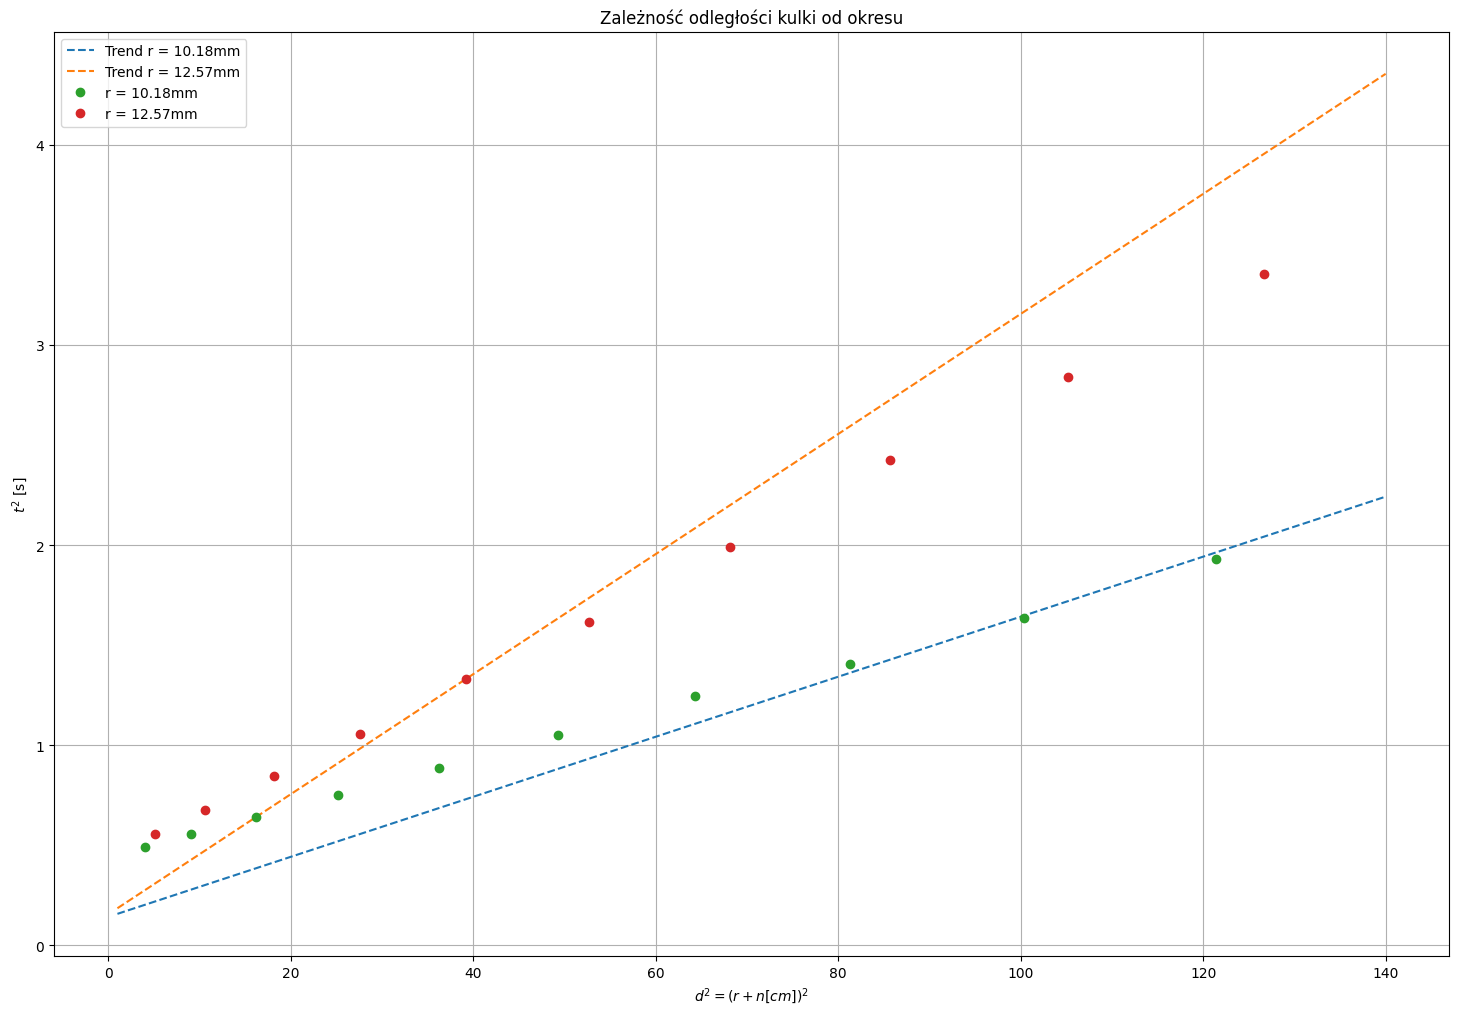
\includegraphics[angle=90, width=\textwidth, height=\textheight, keepaspectratio]{images/sprawozdanie3_2.png}

\pagebreak
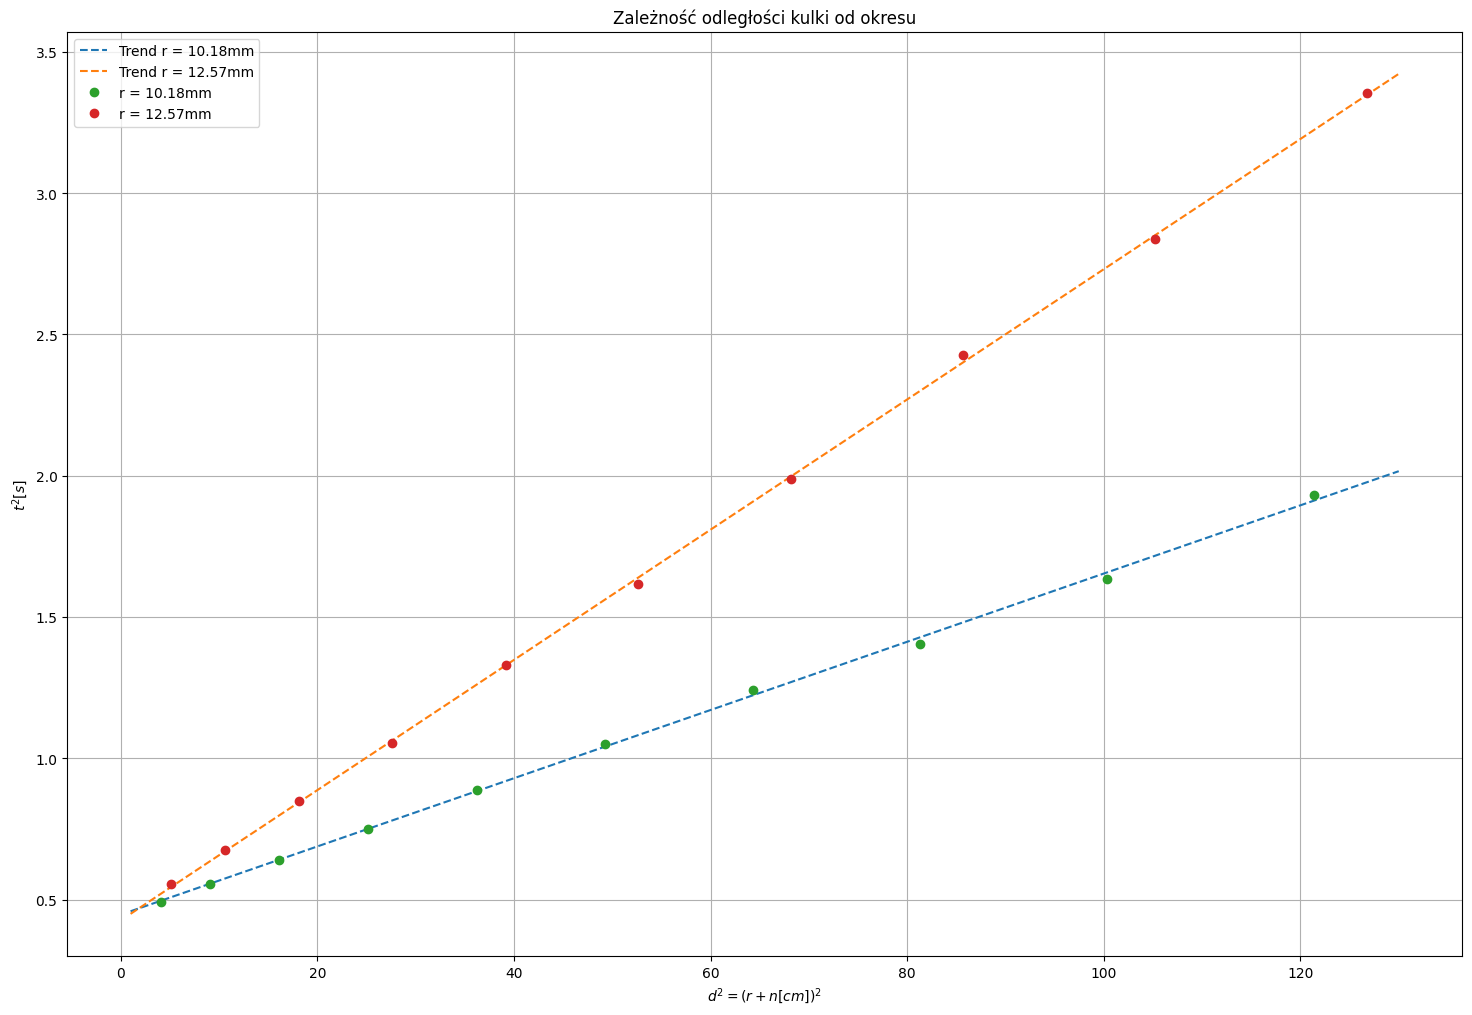
\includegraphics[angle=90, width=\textwidth, height=\textheight, keepaspectratio]{images/sprawozdanie3_3.png}
\end{document}


%Dodatkowe uwagi:

1. Sprawozdanie może być pisane ręcznie. Proszę jednak o czytelność pisma!!!

2. Sprawozdanie MUSI zawierać wszystkie części (tabela pomiarową, teoria,
przebieg ćwiczenia, obliczenia, niepewności, wnioski i wykresy). Brak
jakiejkolwiek części kwalifikuje do zwrotu złożonego sprawozdania bez dalszego
sprawdzania.

3. Wykresy należy zamieszczać na osobnych kartkach (format A4). Wykonywać za
pomocą komputera lub ręcznie na papierze milimetrowym. Należy tak dobrać
skalę, aby wykres zajmował całą stronę.

4. Punktów pomiarowych naniesionych na wykresach nie łączymy! W przypadku
dopasowania prostej regresji, wraz punktami na wykresie należy nanieść prostą
regresji.

5. Na wykresach razem z punktami należy nanieść niepewności pomiarowe w formie
tzw. krzyży niepewności pomiarowych.

6. Do sprawozdania należy dołączyć kartkę pomiarową z ćwiczenia podpisaną przez
prowadzącego.

7. Przy zapisie wyników wraz z niepewnością obowiązuje zasada podawania 2 cyfr
znaczących (instrukcja ONP).

8. Niepewności pomiarowe w większości przypadków wyliczamy bazując na trzech
metodach:
a) gdy mamy pomiary skorelowane korzystamy z zależności 17 w instrukcji ONP,
b) gdy mamy pomiary nieskorelowane korzystamy z zależności 15 w ONP,
c) w przypadku dopasowywania prostych regresji, niepewności obliczamy ze
wzorów 6 i 7 w ONP.